\documentclass[12pt]{article}
\usepackage{url,graphicx,tabularx,array,geometry,enumitem,amsmath}
\setlength{\parskip}{1ex} %--skip lines between paragraphs
\setlength{\parindent}{0pt} %--don't indent paragraphs

%-- Commands for header
\renewcommand{\title}[1]{\textbf{#1}\\}
\renewcommand{\line}{\begin{tabularx}{\textwidth}{X>{\raggedleft}X}\hline\\\end{tabularx}\\[-0.5cm]}
\newcommand{\leftright}[2]{\begin{tabularx}{\textwidth}{X>{\raggedleft}X}#1%
& #2\\\end{tabularx}\\[-0.5cm]}

%\linespread{2} %-- Uncomment for Double Space
\begin{document}

\title{Digital Signal Processing - Assignment 2}
\line
\leftright{\today}{Stephanie Lund (2555914)\\Aljoscha Dietrich(2557976)} %-- left and right positions in the header

\section*{Exercise 1}

\begin{enumerate}[label=\alph*)]
\item 
$\begin{aligned}[t]
X(e^{j\omega}) &= \sum_{n=-\infty}^{\infty} x[n]e^{-j\omega n}\\
&= \sum_{n=-\infty}^{-1} x[n]e^{-j\omega n} + \sum_{n=0}^{3} x[n]e^{-j\omega n} + \sum_{n=4}^{\infty} x[n]e^{-j\omega n} \\
&=  \sum_{n=0}^{3} x[n]e^{-j\omega n} \\
&= 1 + e^{-j\omega} + e^{-j2\omega} + e^{-j3\omega}\\
\end{aligned}$
\\ \\
\item 
$\begin{aligned}[t]
X[k] &= \sum_{n=0}^{N-1} x[n]W_{N}^{kn}\\
&= \sum_{n=0}^{N-1} x[n](e^{-j\frac{2\pi}{N}})^{kn} \\
&= \sum_{n=0}^{3} x[n] (e^{-j\frac{2\pi}{N}})^{kn} \\
&= 1 + (e^{-j\frac{2\pi}{N}})^{k} + (e^{-j\frac{2\pi}{N}})^{2k} + (e^{-j\frac{2\pi}{N}})^{3k}
\end{aligned}$

\item If we take $N$ samples from the formula in part $a)$, then $\omega = \frac{2\pi}{N}k$
\begin{align*}
X(e^{j\omega}) &= 1 + e^{-j\omega} + e^{-j2\omega} + e^{-j3\omega}\\
&= 1 + (e^{-j\frac{2\pi}{N}})^{k} + (e^{-j\frac{2\pi}{N}})^{2k} + (e^{-j\frac{2\pi}{N}})^{3k}
\end{align*}

\end{enumerate}

\section*{Exercise 2}

\begin{enumerate}[label=\alph*)]

\item The highest frequency, given by $5cos(50\pi t)$, is 25. The minimum sampling rate must be at least twice the highest frequency, so it would need to be greater than 50.

\item $f_s = 25$. Then $t = \frac{k}{25}$ (where $k$ is an integer), and:
\begin{align*}
y(t) &= 10cos(20\pi t - \frac{\pi}{4}) - 5cos(50\pi t)\\
&= 10cos(20\pi t - \frac{\pi}{4}) - 5cos(50\pi \frac{k}{25}) \\
&= 10cos(20\pi t - \frac{\pi}{4}) - 5cos(2\pi k) \\
&= 10cos(20\pi t - \frac{\pi}{4}) - 5 \\
\end{align*}

\item As shown above, $A = -5$

\end{enumerate}

\section*{Exercise 3}
\begin{tabular}{*{8}{| c }|}
\hline
$W_2^0$ & & & & $W_2^1$ & & & \\
\hline
$W_4^0$ & & $W_4^1$ & & $W_4^2$ & & $W_4^3$ & \\
\hline
$W_8^0$ & $W_8^1$ & $W_8^2$ & $W_8^3$ & $W_8^4$ & $W_8^5$ & $W_8^6$ & $W_8^7$ \\
\hline
1 & $\frac{\sqrt[]{2}}{2} - \frac{\sqrt[]{2}}{2}i$ & $-i$ & $-\frac{\sqrt[]{2}}{2} - \frac{\sqrt[]{2}}{2}i$ & -1 & $-\frac{\sqrt[]{2}}{2} + \frac{\sqrt[]{2}}{2}i$ & $i$ & $\frac{\sqrt[]{2}}{2} + \frac{\sqrt[]{2}}{2}i$ \\
\hline
\end{tabular}


\begin{tabular}{*{8}{|c}|}
\hline
$p_{11}$ & $p_{12}$ & $p_{13}$ & $p_{14}$ & $p_{15}$ & $p_{16}$ & $p_{17}$ & $p_{18}$ \\
\hline
2 & 0 & 2 & 0 & 2 & 0 & 2 & 0\\
\hline
\end{tabular}

\begin{tabular}{*{8}{|c}|}
\hline
$p_{21}$ & $p_{22}$ & $p_{23}$ & $p_{24}$ & $p_{25}$ & $p_{26}$ & $p_{27}$ & $p_{28}$ \\
\hline
4 & 0 & 0 & 0 & 4 & 0 & 0 & 0\\
\hline
\end{tabular}

\begin{tabular}{*{8}{|c}|}
\hline
$S_0$ & $S_1$ & $S_2$ & $S_3$ & $S_4$ & $S_5$ & $S_6$ & $S_7$ \\
\hline
8 & 0 & 0 & 0 & 0 & 0 & 0 & 0\\
\hline
\end{tabular}


\section*{Exercise 4}
\begin{enumerate}[label=\alph*)]
\item 
$\begin{aligned}[t]
y[0] &= h[0]x[0] = 0.5 \cdot 1.0 = 0.5 \\
y[1] &= h[0]x[1] + h[1]x[0] = 0.5 \cdot 2.0 + 0.5\cdot 1.0 = 1.5 \\
y[2] &= h[0]x[2] + h[1]x[1] + h[2]x[0] = 0.5\cdot2.0 = 1.0 \\
y[n] &= [0.5\quad1.5\quad1.0]
\end{aligned}$

\item
$\begin{aligned}[t]
H(e^{-j\omega}) &= \sum_{n=-\infty}^{\infty} h(n) \cdot e^{-i \omega n} = h(0) + h(1) \cdot e^{-i\omega} = \frac{1}{2}\cdot[1 + e^{-j\omega}]
\end{aligned}$

\item 
$\begin{aligned}[t]
A(\omega) &= \lvert H(e^{-j\omega}) \rvert \\
&= \lvert \frac{1}{2}\cdot[1 + e^{-j\omega}] \rvert \\
&= \frac{1}{2} \lvert 1 + cos(-\omega) + i sin(-\omega) \rvert \\
&= \frac{1}{2} \sqrt[]{(1 + cos(\omega))^2 + sin(\omega)^2} \\
&= \frac{1}{2} \sqrt[]{1 + cos^2(\omega) + 2cos(\omega) + sin^2(\omega)} \\
&= \frac{1}{2} \sqrt[]{2 + 2cos(\omega)} \\
&= \frac{1}{2} \sqrt[]{4(\frac{1 + cos(\omega)}{2})} \\
&= cos(\frac{\omega}{2})
\end{aligned}$

Then, for $\omega = 2\pi f$, the amplitude response as a function of $f$ is $cos(\frac{2\pi f}{2})$ and looks as follows:\\\\
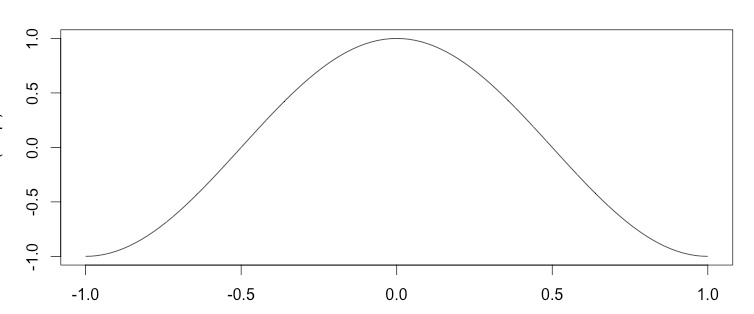
\includegraphics[scale=0.55]{hw2-img.png}

\end{enumerate}


\end{document}
